\begin{Example}[mental4]{Mental impairment and parents' SES}
We consider here adjacent category logit models for the Mental Health
data, treating \pname{MENTAL} as an ordinal response.
Adjacent logit models are easily fit with \PROC{CATMOD}
using the \pname{RESPONSE ALOGIT;} statement.
Differences among the logits for adjacent categories (the intercepts, $\beta_j$, in models \eqref{eq:alin} and \eqref{eq:arow}) are
specified by the \verb|_RESPONSE_| keyword in the
\stmt{MODEL}{CATMOD}.  Nominal explanatory variables are included
as main effects (and possibly, interactions) on the left-hand side
of the \stmt{MODEL}{CATMOD}.  An explanatory variable is treated
as quantitative when declared in a \stmt{DIRECT}{CATMOD}.

The following statements fit a series of adjacent category logit models
to the Mental Health data.  Model 0 has only a \verb|_RESPONSE_|
effect, and is analogous to the independence model.
In Model 1, the adjacent logits for mental impairment are affected
by SES, as a nominal variable.
Model 2 is the linear-by-linear model for adjacent logits, with
SES as a direct variable,
while Model 3 allows different slopes for each adjacent logit.
%% input: /users/faculty/friendly/sasuser/catdata/mental4.sas
%% last modified: 01-Dec-98 12:07
\begin{listing}
%include catdata(mental);

*-- Adjacent logit models;
proc catmod data=mental;
   weight count;
   population ses;
   response alogit / out=pred0;
   model mental = _response_ / noprofile noresponse title='Model 0:  _R_';
  run;
   response alogit / out=pred1;
   model mental = _response_  ses / noprofile noresponse title='Model 1: _R_ SES';
  run;
   direct ses;
   response alogit / out=pred2;
   model mental = _response_  ses / noprofile noresponse title='Model 2: _R_ S';
  run;
   direct ses;
   response alogit / out=pred3;
   model mental = _response_ | ses / noprofile noresponse title='Model 3: _R_|S';
  run;
\end{listing}

%% two subfig side-by-side
\begin{figure}[htb]
 \begin{minipage}[t]{.49\linewidth}
  \includegraphics[width=1\linewidth]{mental41}
 \end{minipage}%
 \hfill
 \begin{minipage}[t]{.49\linewidth}
  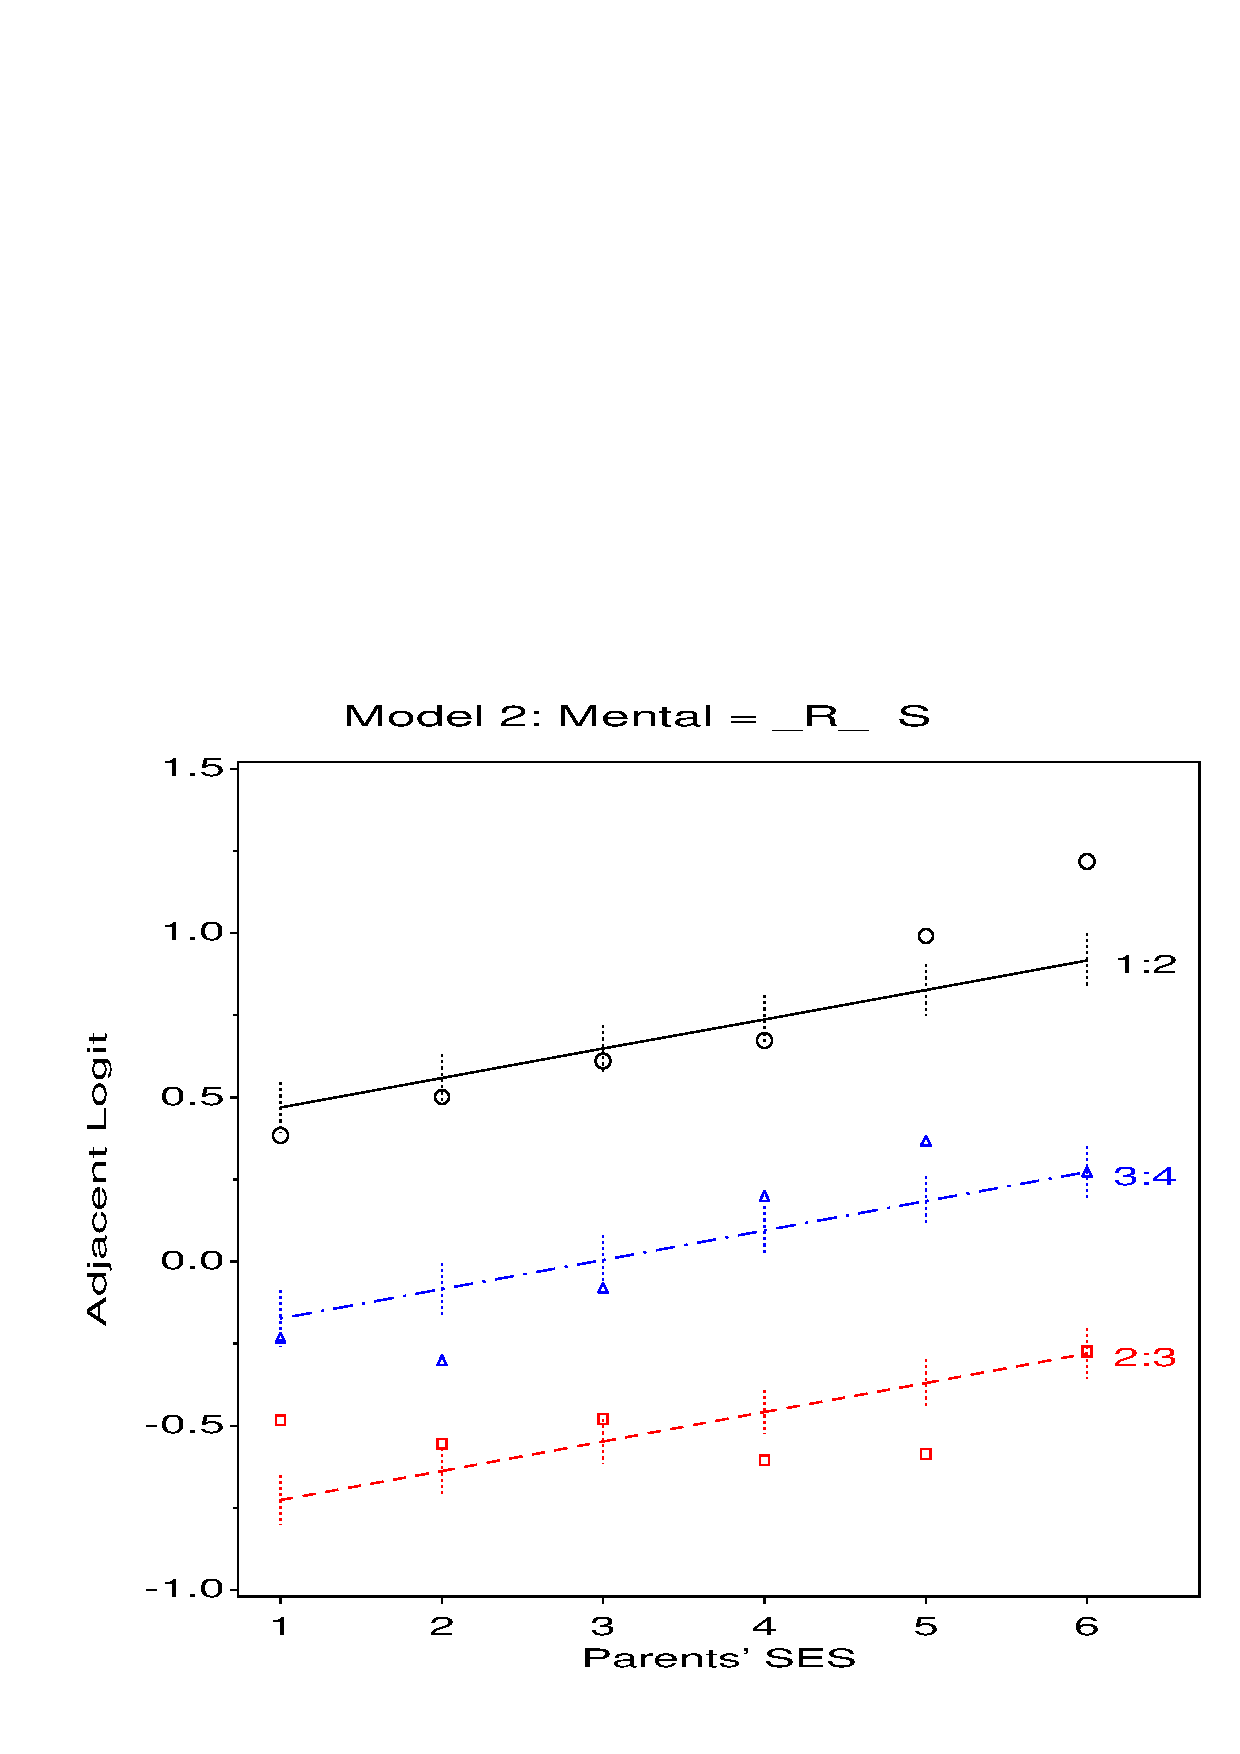
\includegraphics[width=1\linewidth]{mental42}
 \end{minipage}
 \caption{Adjacent category logit models for Mental Health data, Model 1 and Model 2}\label{fig:mental4a}
\end{figure}
\begin{table}[htb]
 \caption{Adjacent category logit models for Mental Health data}\label{tab:mentab4}
 \begin{center}
 \renewcommand{\arraystretch}{1.1}
 \begin{tabular}{c ll rrr r}
  \hline
  Model & Formula & Terms & df & \chisq\ & $p$-value & AIC\\ 
  \hline
  0 & $A_{j| i} = \beta_j $                  & \verb\_R_\     & 15 & 44.35 & 0.0001 & 14.35\\ 
  1 & $A_{j| i} = \beta_j + \alpha_i$        & \verb\_R_ SES\ & 10 & 6.76 & 0.7478  & -13.24\\ 
  2 & $A_{j| i} = \beta_j + \gamma \: a_i$   & \verb\_R_ S\   & 14 & 9.68 & 0.7849  & -18.32\\ 
  3 & $A_{j| i} = \beta_j + \gamma_j a_i$    & \verb\_R_|S\   & 12 & 6.26 & 0.9023 & -17.74\\ 
  4 & $A_{j| i} = \beta_j + \gamma_1 a_i + \gamma_2 a_i^2$ & \verb\_R_ S S^2\ & 13 & 7.39 & 0.8809 & -18.61\\ 
  5 & $A_{j| i} = \beta_j + \gamma_j a_i + \delta a_i^2$ & \verb\_R_|S S^2\ & 11 & 3.69 & 0.9782 & -18.69\\ 
  \hline
 \end{tabular}
 \end{center}
\end{table}

For each model, an \ODS, which contains the observed and fitted logits,
is requested with the \opt{OUT=}{CATMOD} in the \stmt{RESPONSE}{CATMOD}.
Plotting the observed and fitted logits
makes it easy to see what relationships are implied by each model.
The plots for Model 1 and Model 2, shown in \figref{fig:mental4a},
are produced with the \macro{CATPLOT}
as shown below.
The macro call requests a plot of the observed logit
(\verb|_OBS_|) against \pname{SES}, with separate curves for each
adjacent logit (\verb|CLASS=_NUMBER_|).
By default, the macro also draws curves connecting the predicted
values (\verb|_PRED_| in the \ODS) and $\pm 1$ standard error bars
around each fitted logit.
\begin{listing}
axis1 label=(a=90) order=(-1 to 1.5 by .5);
axis2 offset=(3,8);
proc format;
   value cum 1='1:2'  2='2:3'  3='3:4';
title 'Model 1: Mental = _R_ SES';
%catplot(data=pred1, x=ses, y=_obs_, class=_number_, clfmt=cum.,
   type=FUNCTION, ylab=Adjacent Logit);

title 'Model 2: Mental = _R_  S';
%catplot(data=pred2, x=ses, y=_obs_, class=_number_, clfmt=cum.,
   type=FUNCTION, ylab=Adjacent Logit);
\end{listing}

For illustration, we also fit less restrictive models,
allowing a quadratic relation between the adjacent logit and SES (Model 4).
Model 5 adds a quadratic term
to the unequal slopes allowed in Model 3.
Plots for Model 3 and Model 5 are shown in \figref{fig:mental4b}.
%% input: /Users/friendly/sasuser/catdata/mental4.sas
%% last modified: 19-Aug-99 11:31
\begin{listing}
proc catmod data=mental;
   weight count;
   population ses;
   direct ses;
   response alogit / out=pred4;
   model mental = _response_ ses ses*ses / noprofile noiter title='Model 4: _R_ S S^2';
  run;
   response alogit / out=pred5;
   model mental = _response_|ses ses*ses / noprofile noiter title='Model 5: _R_|S S^2';
  run;
\end{listing}


%% two subfig side-by-side
\begin{figure}[htb]
 \begin{minipage}[t]{.49\linewidth}
  \includegraphics[width=1\linewidth]{mental43}
 \end{minipage}%
 \hfill
 \begin{minipage}[t]{.49\linewidth}
  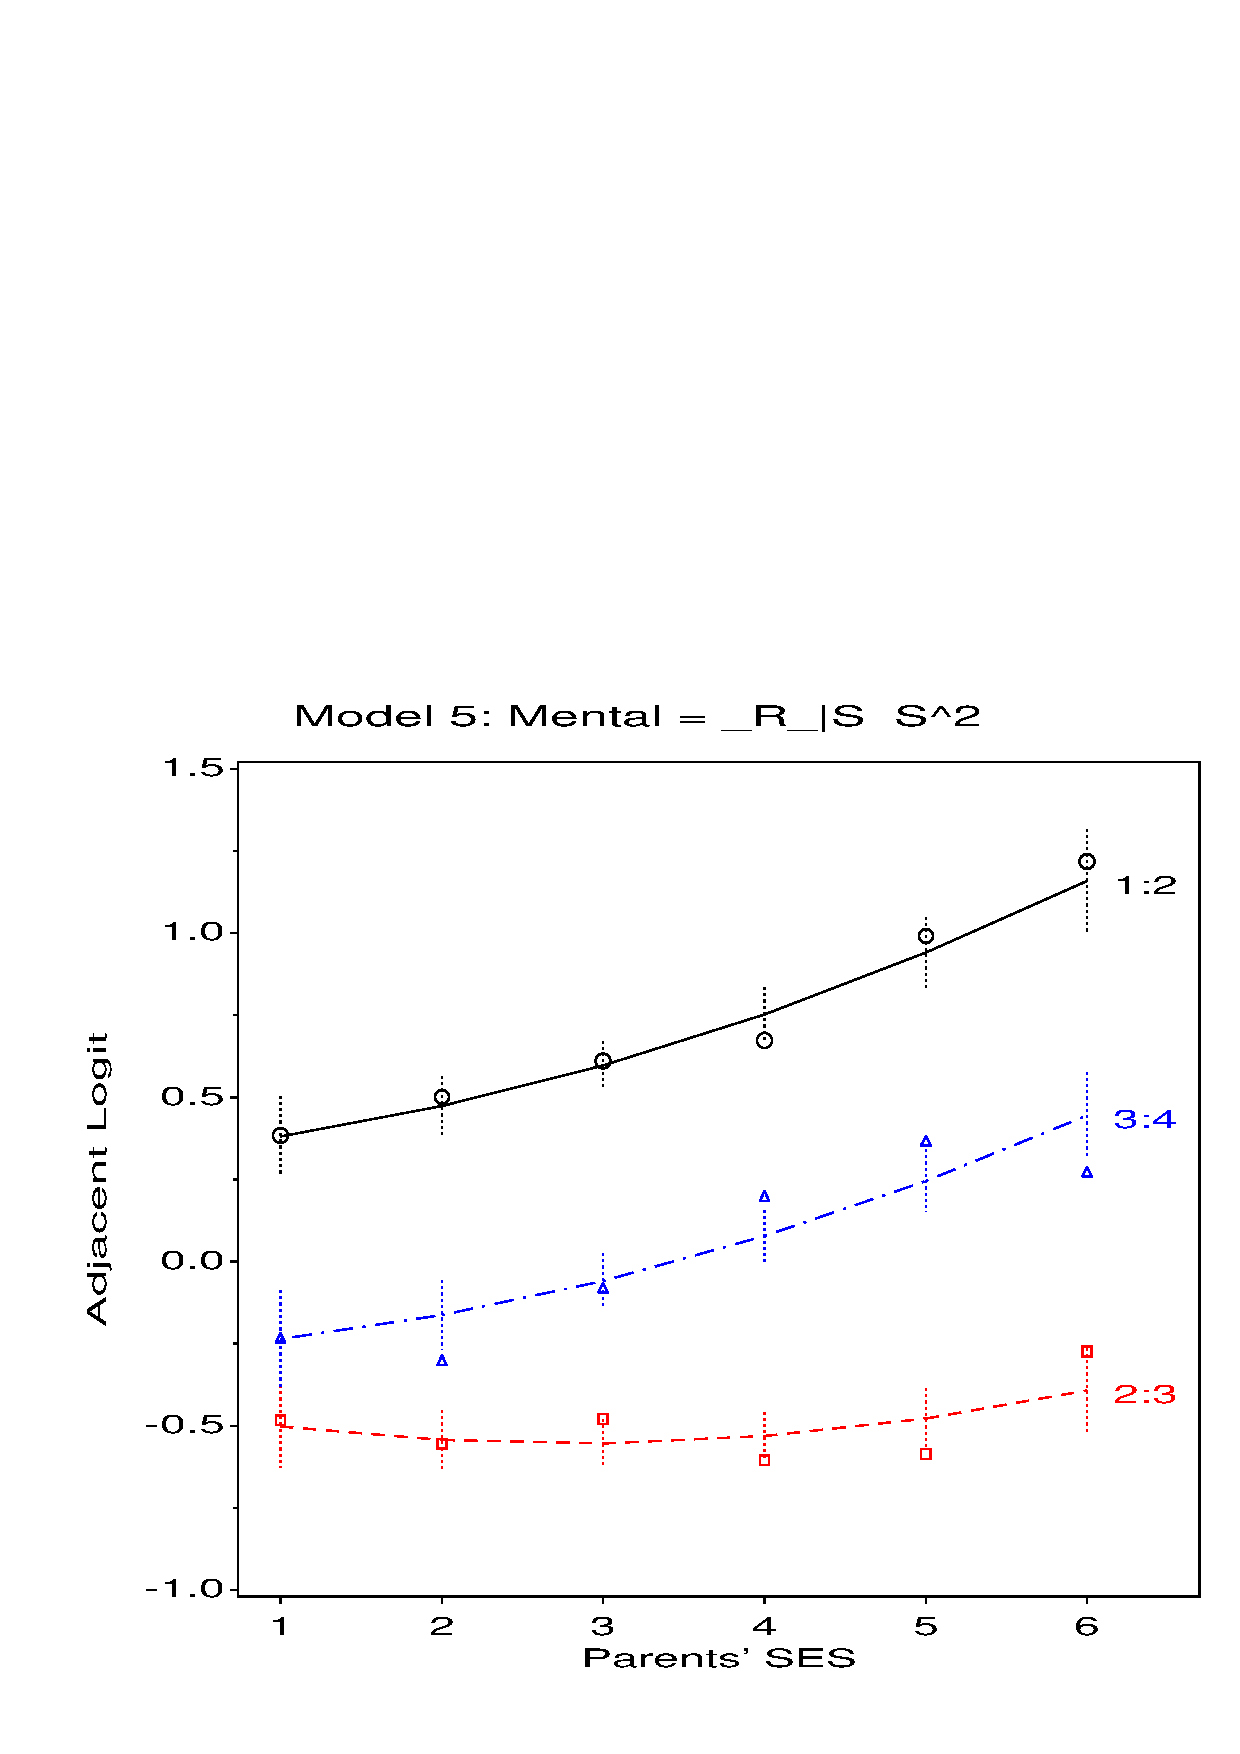
\includegraphics[width=1\linewidth]{mental44}
 \end{minipage}
 \caption{Adjacent category logit models for Mental Health data: Model 3 and Model 5}\label{fig:mental4b}
\end{figure}

What may we conclude from this?
From \tabref{tab:mentab4}, all models except the independence model
have acceptable fit according to the \chisq\ values;
Models 2--5 all have smaller AIC values than Model 1;  of these,
Model 2, the linear-by-linear is the most parsimonious, but Models
4 and 5 have slightly smaller AIC values.

One interpretation, from the plots in \figref{fig:mental4a} and \figref{fig:mental4b}
is that there is evidence that not both of SES and mental impairment
can be considered linear with unit spacing.
The intercepts suggest that the gap between categories 1 and 2
(`Well', 'Mild impairment') is greatest on the mental health scale,
and that between categories 2 and 3 (`Mild', `Moderate impairment')
is smallest.
The evidence regarding the metric for SES is more ambiguous:
there is a suggestion of a mildly quadratic relationship with SES,
particularly for the logit between response categories 1 and 2,
but this may be due to the points for (lowest) SES categories 5 and 6,
where the large logit values imply
a relatively larger number of people
classified as mildly impaired as opposed to well.
\end{Example}
